\documentclass[a4paper,11pt]{ltjsarticle}
\usepackage[haranoaji]{luatexja-preset}
\usepackage{amsmath,amssymb}
\usepackage[top=12mm,bottom=10mm,left=14mm,right=14mm]{geometry}
\usepackage{array}
\usepackage{tikz}
\usetikzlibrary{calc}
\pagestyle{empty}
\setlength{\parindent}{0pt}
\newlength{\qcol}\setlength{\qcol}{0.47\textwidth}
\newlength{\qgap}
\newlength{\anscolw}\setlength{\anscolw}{0.30\textwidth}
\newlength{\ansh}
\newcommand{\Q}[2]{\parbox[t]{\qcol}{\raggedright (#1)\hspace{0.6em}$\displaystyle #2$}}
\newcommand{\QR}[4]{\Q{#1}{#2}\hfill\Q{#3}{#4}\par\vspace{\qgap}}
\newcommand{\anscell}[1]{\rule[-\ansdrop]{0pt}{\ansh}(#1)}
\newlength{\ansdrop}

\begin{document}
{\large\bfseries 数学テスト　3}\hfill 名前(\underline{\hspace{32mm}})\par\vspace{3mm}
■（1）〜（12）の計算をしなさい。（13）、（14）は連立方程式を解きなさい。\par\vspace{3mm}
\setlength{\qgap}{11mm}
\QR{1}{(-4a)^3}{2}{(32x+12y)\div4}
\QR{3}{\dfrac{a-3b}{3}-\dfrac{2a-b}{5}}{4}{2a-\{7b-(4a+3b)+5\}}
\QR{5}{12a^2b\div3a}{6}{(3x+4y)-(2x-3y)-(5x+2y)}
\QR{7}{3a^2\times(-2a)}{8}{2(a-3b)-3(a-2b)}
\QR{9}{(5x-3y)+(-4x+6y)}{10}{(4a^2-3a-1)+(-2a^2+5a+6)}
\QR{11}{\dfrac{3}{4}(12x-8y)}{12}{6a^3b^2\div3ab\times2a}
\QR{13}{\left\{\begin{array}{l} x=y-1 \\ 3x-2y=1 \end{array}\right.}{14}{\left\{\begin{array}{l} 5x-2y=19 \\ 4x+5y=2 \end{array}\right.}
\vspace{2mm}
\setlength{\ansh}{11mm}\setlength{\ansdrop}{7mm}%
\begin{center}\begin{tabular}{|p{\anscolw}|p{\anscolw}|p{\anscolw}|}\hline
\anscell{1} & \anscell{2} & \anscell{3} \\\hline
\anscell{4} & \anscell{5} & \anscell{6} \\\hline
\anscell{7} & \anscell{8} & \anscell{9} \\\hline
\anscell{10} & \anscell{11} & \anscell{12} \\\hline
\anscell{13} & \anscell{14} &  \\\hline
\end{tabular}\end{center}

\newpage

\begin{minipage}[t]{0.56\textwidth}
(3)　右の図2で，$\ell /\!/ m$ である。㋑の角の大きさは\par
\hspace*{1.2em}何度か，求めよ。\par\vspace{6mm}
答(\underline{\hspace{28mm}})
\end{minipage}\hfill
\begin{minipage}[t]{0.40\textwidth}
{\bfseries 図2}\par\vspace{2mm}
\scalebox{0.72}{
\begin{tikzpicture}[scale=1.15,line width=0.5pt]
  \coordinate (P) at (3,0);
  \coordinate (Q) at (2.32,1.88);
  \coordinate (R) at (6.27,3.30);
  \draw (1.3,3.30) -- (7.6,3.30);
  \node[left] at (1.3,3.30) {$\ell$};
  \draw (1.3,0) -- (7.6,0);
  \node[left] at (1.3,0) {$m$};
  \draw (P) -- (Q) -- ($(R)+(0.75,0.27)$);
  \draw ($(Q)+(0.20,0.07)$) -- ($(Q)+(0.20,0.07)+(-0.07,0.20)$) -- ($(Q)+(-0.07,0.20)$);
  \draw (P)+(0.7,0) arc (0:110:0.7);
  \node[anchor=west,fill=white,inner sep=1.5pt] at (3.62,0.52) {$110^\circ$};
  \draw ($(R)+(-0.75,0)$) arc (180:207:0.75);
  \node[fill=white,inner sep=1pt] at (5.62,2.72) {㋑};
\end{tikzpicture}
}
\end{minipage}
\par\vspace{12mm}
\begin{minipage}[t]{0.56\textwidth}
(5)　右の図3は，円柱を平面で2つに切り分けた\par
\hspace*{1.2em}ときにできた立体である。\par
\hspace*{1.2em}この立体の体積は何 $\mathrm{cm}^3$ か，求めよ。\par\vspace{6mm}
答(\underline{\hspace{28mm}})
\end{minipage}\hfill
\begin{minipage}[t]{0.40\textwidth}
{\bfseries 図3}\par\vspace{2mm}
\hspace*{6mm}
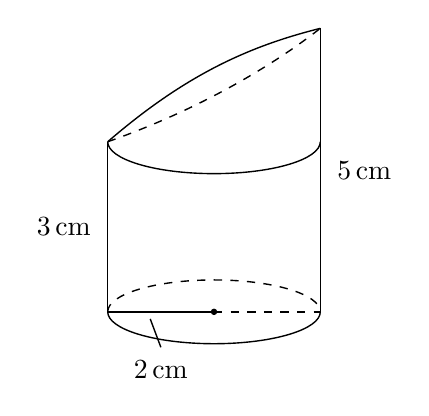
\begin{tikzpicture}[scale=0.9,line width=0.5pt]
  \draw (-1.5,0) arc (180:360:1.5 and 0.45);
  \draw[dashed] (-1.5,0) arc (180:0:1.5 and 0.45);
  \draw (-1.5,0) -- (-1.5,2.4);
  \draw (1.5,0) -- (1.5,4.0);
  \draw (-1.5,2.4) arc (180:360:1.5 and 0.45);
  \draw (-1.5,2.4) .. controls (-0.4,3.35) and (0.5,3.75) .. (1.5,4.0);
  \draw[dashed] (-1.5,2.4) .. controls (-0.5,2.75) and (0.6,3.3) .. (1.5,4.0);
  \fill (0,0) circle (1.3pt);
  \draw (-1.5,0) -- (0,0);
  \draw[dashed] (0,0) -- (1.5,0);
  \node[left] at (-1.6,1.2) {3\,cm};
  \node[right] at (1.6,2.0) {5\,cm};
  \node[below] at (-0.75,-0.55) {2\,cm};
  \draw (-0.75,-0.5) -- (-0.9,-0.1);
\end{tikzpicture}

\end{minipage}

\end{document}
